\chapter{第一个项目：调试项目}
\label{ch:concise-debug}

\begin{introduction}
  \item 新建调试项目并填写测试序列；
  \item 完成配置检查、编译与烧录；
  \item 用提示音与逐项观察确认每一路输出。
\end{introduction}

调试项目不读取遥控器，也不涉及底盘、云台与拨弹逻辑。它只按顺序启停主控板上的输出，
适合在装车之前验证接线、供电、电机转向与烧录链路，是第一次使用 PIE-Block 的首选。

\section{新建项目}

从首页“新建项目”开始，项目类型选择“调试”，填写项目名称与保存位置后创建。向导共四步：
测试序列、检查与摘要、生成代码、烧录。

\section{填写测试序列}

“测试序列”页列出主控板能够控制的十路输出，每一路都有独立开关（图~\ref{fig:concise-debug-tests}）。
只有打开的项才会写入固件，关闭的项整段跳过。

\begin{figure}[htbp]
  \centering
  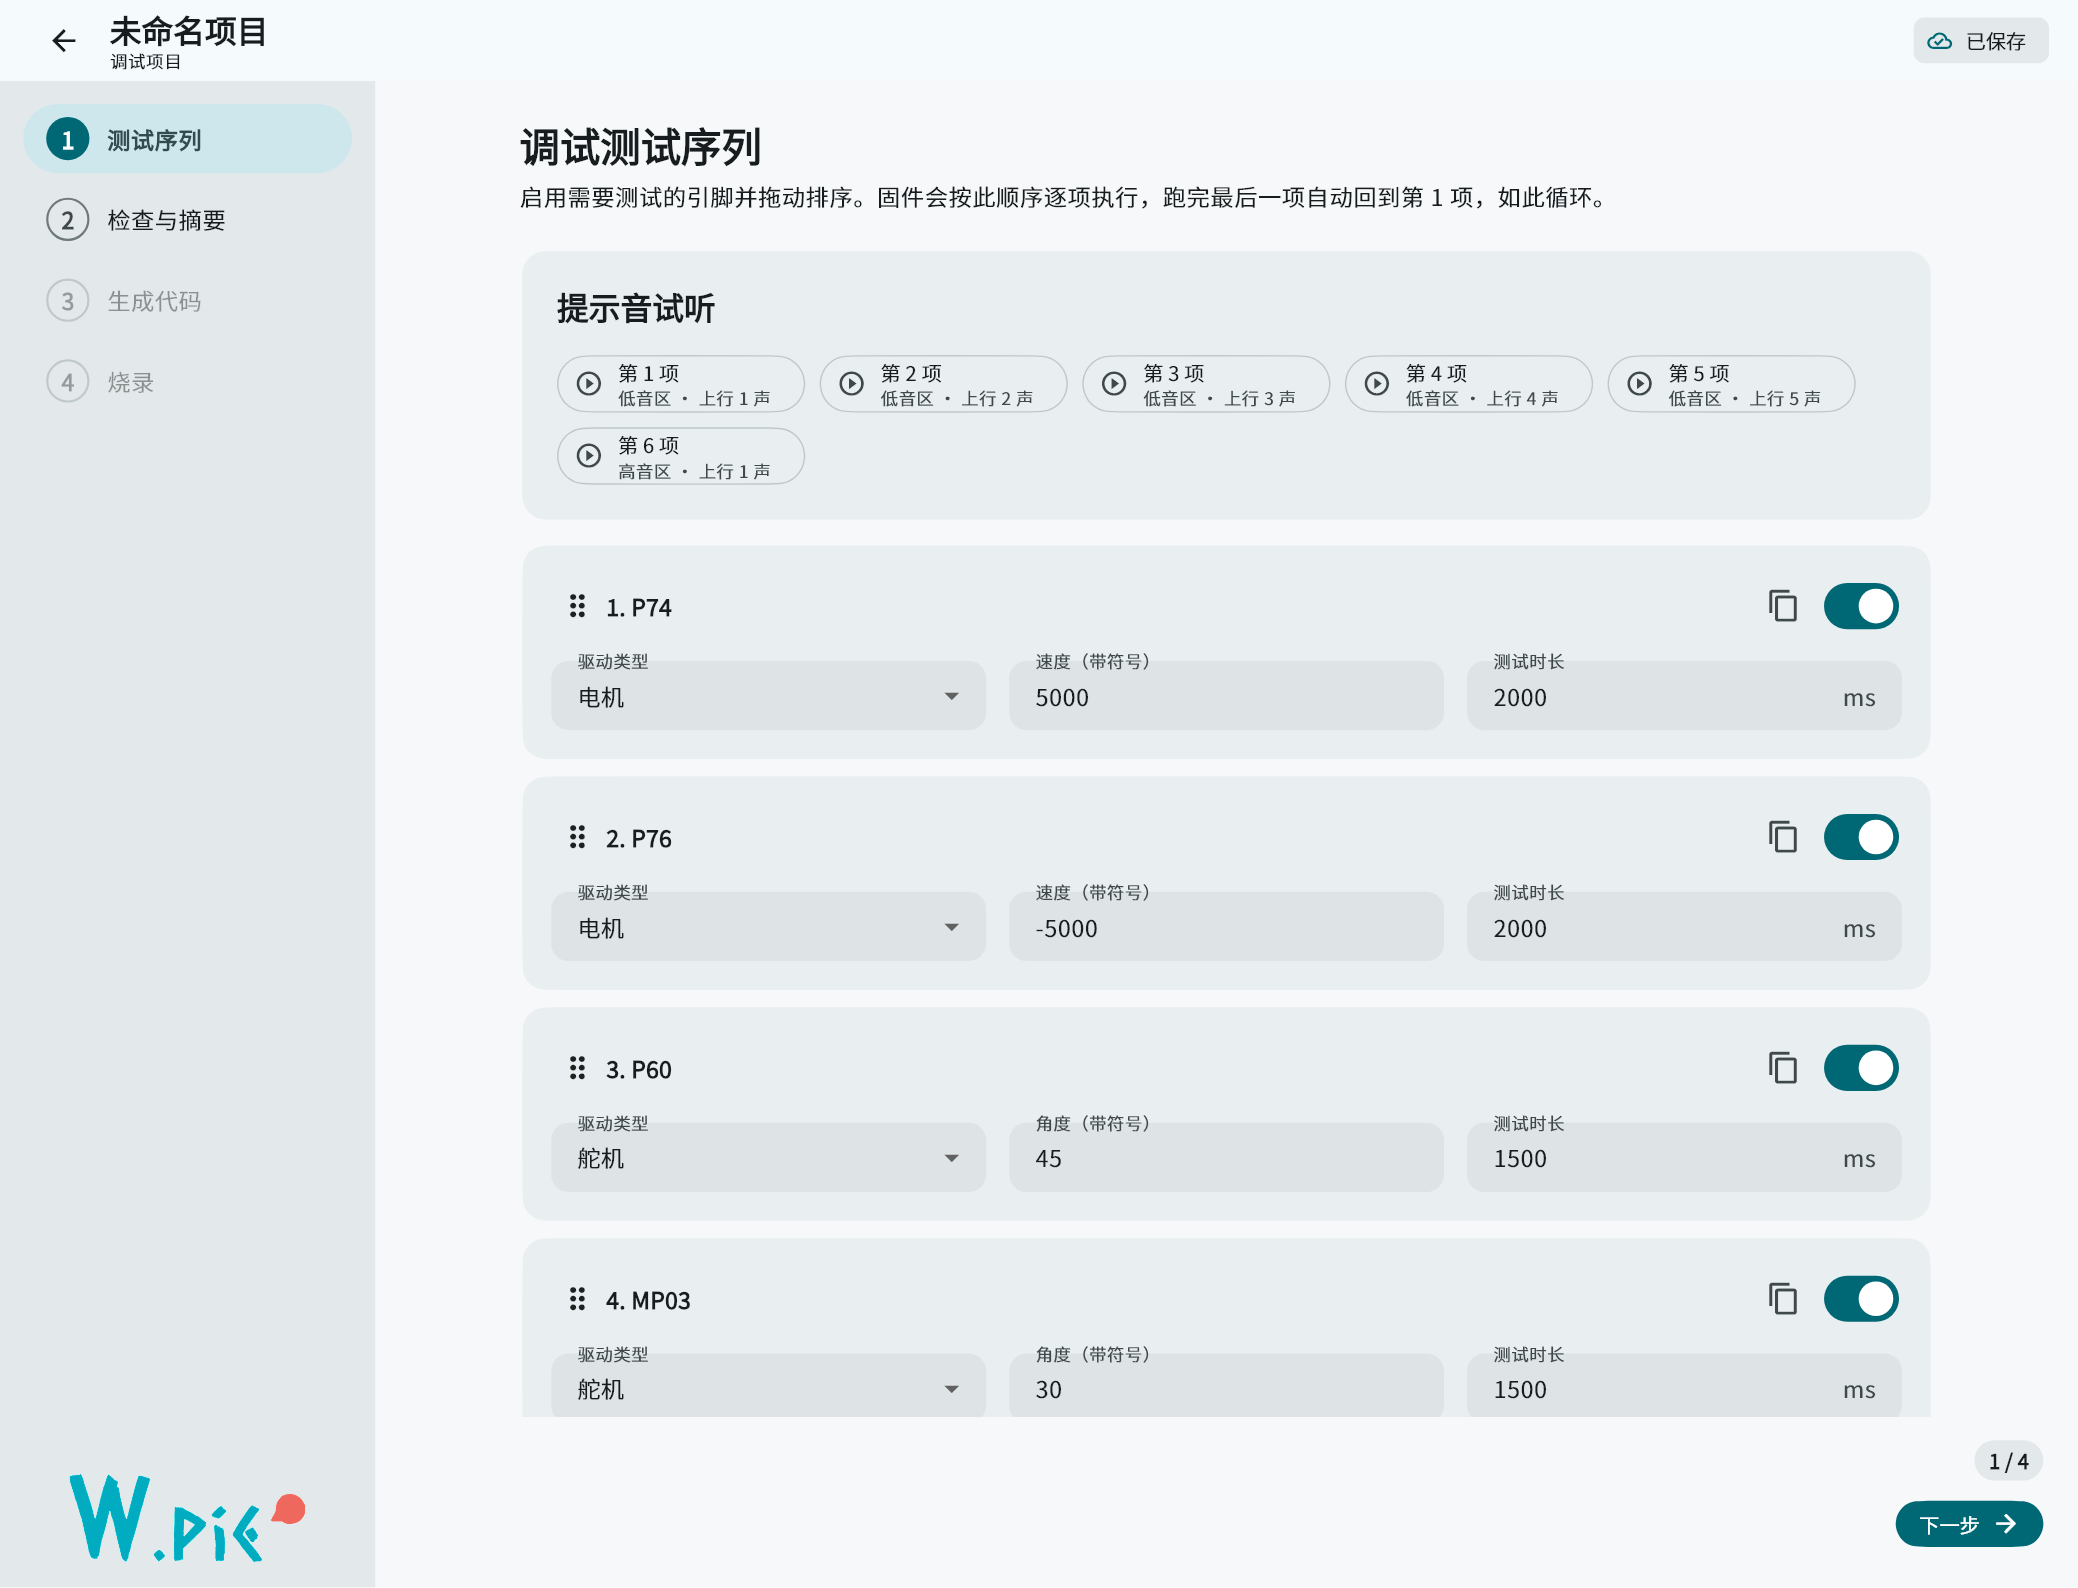
\includegraphics[width=0.95\linewidth]{image/ch06/6-1-debug-tests.png}
  \caption{调试项目的“测试序列”页：上方为提示音试听，下方为按执行顺序排列的测试项}
  \label{fig:concise-debug-tests}
\end{figure}

每个启用的测试项按驱动类型填写：

\begin{itemize}
  \item \textbf{电机}：速度（带符号）与测试时长。正数按默认方向，负数反向，用于在不改
        接线的情况下纠正转向；
  \item \textbf{舵机}：角度（带符号）与测试时长。角度相对中位，方向由正负号决定；
  \item \textbf{摩擦轮}：仅在摩擦轮端口可选，填写目标转速，不填时长。摩擦轮项自带启动
        与渐变流程，执行时自动完成。
\end{itemize}

左侧的拖动手柄用于调整顺序，固件按列表顺序逐项执行，每项结束输出归零，跑完最后一项
自动回到第 1 项循环。需要分段验证同一路时，点击该项右侧的复制键，在下方插入一条相同
配置，再修改数值或时长即可。

装车检查建议按“从轮子到武器”的顺序排列：四个轮电机、云台舵机、摩擦轮。摩擦轮放在最后，
前面任何一项异常都可以直接断电。

页面上方的“提示音试听”把第 $N$ 项对应到上行音型的第 $N$ 个音。装车后即使看不到屏幕，
也可以凭声音判断当前执行到第几项。

\section{检查与摘要}

点击“下一步”进入“检查与摘要”页（图~\ref{fig:concise-debug-review}）。检查结果分为错误与
警告：错误阻止生成，警告只作提示。示例配置只有一项，结果为 0 错误、0 警告，页面提示
“配置检查通过，可以生成代码”。

\begin{figure}[htbp]
  \centering
  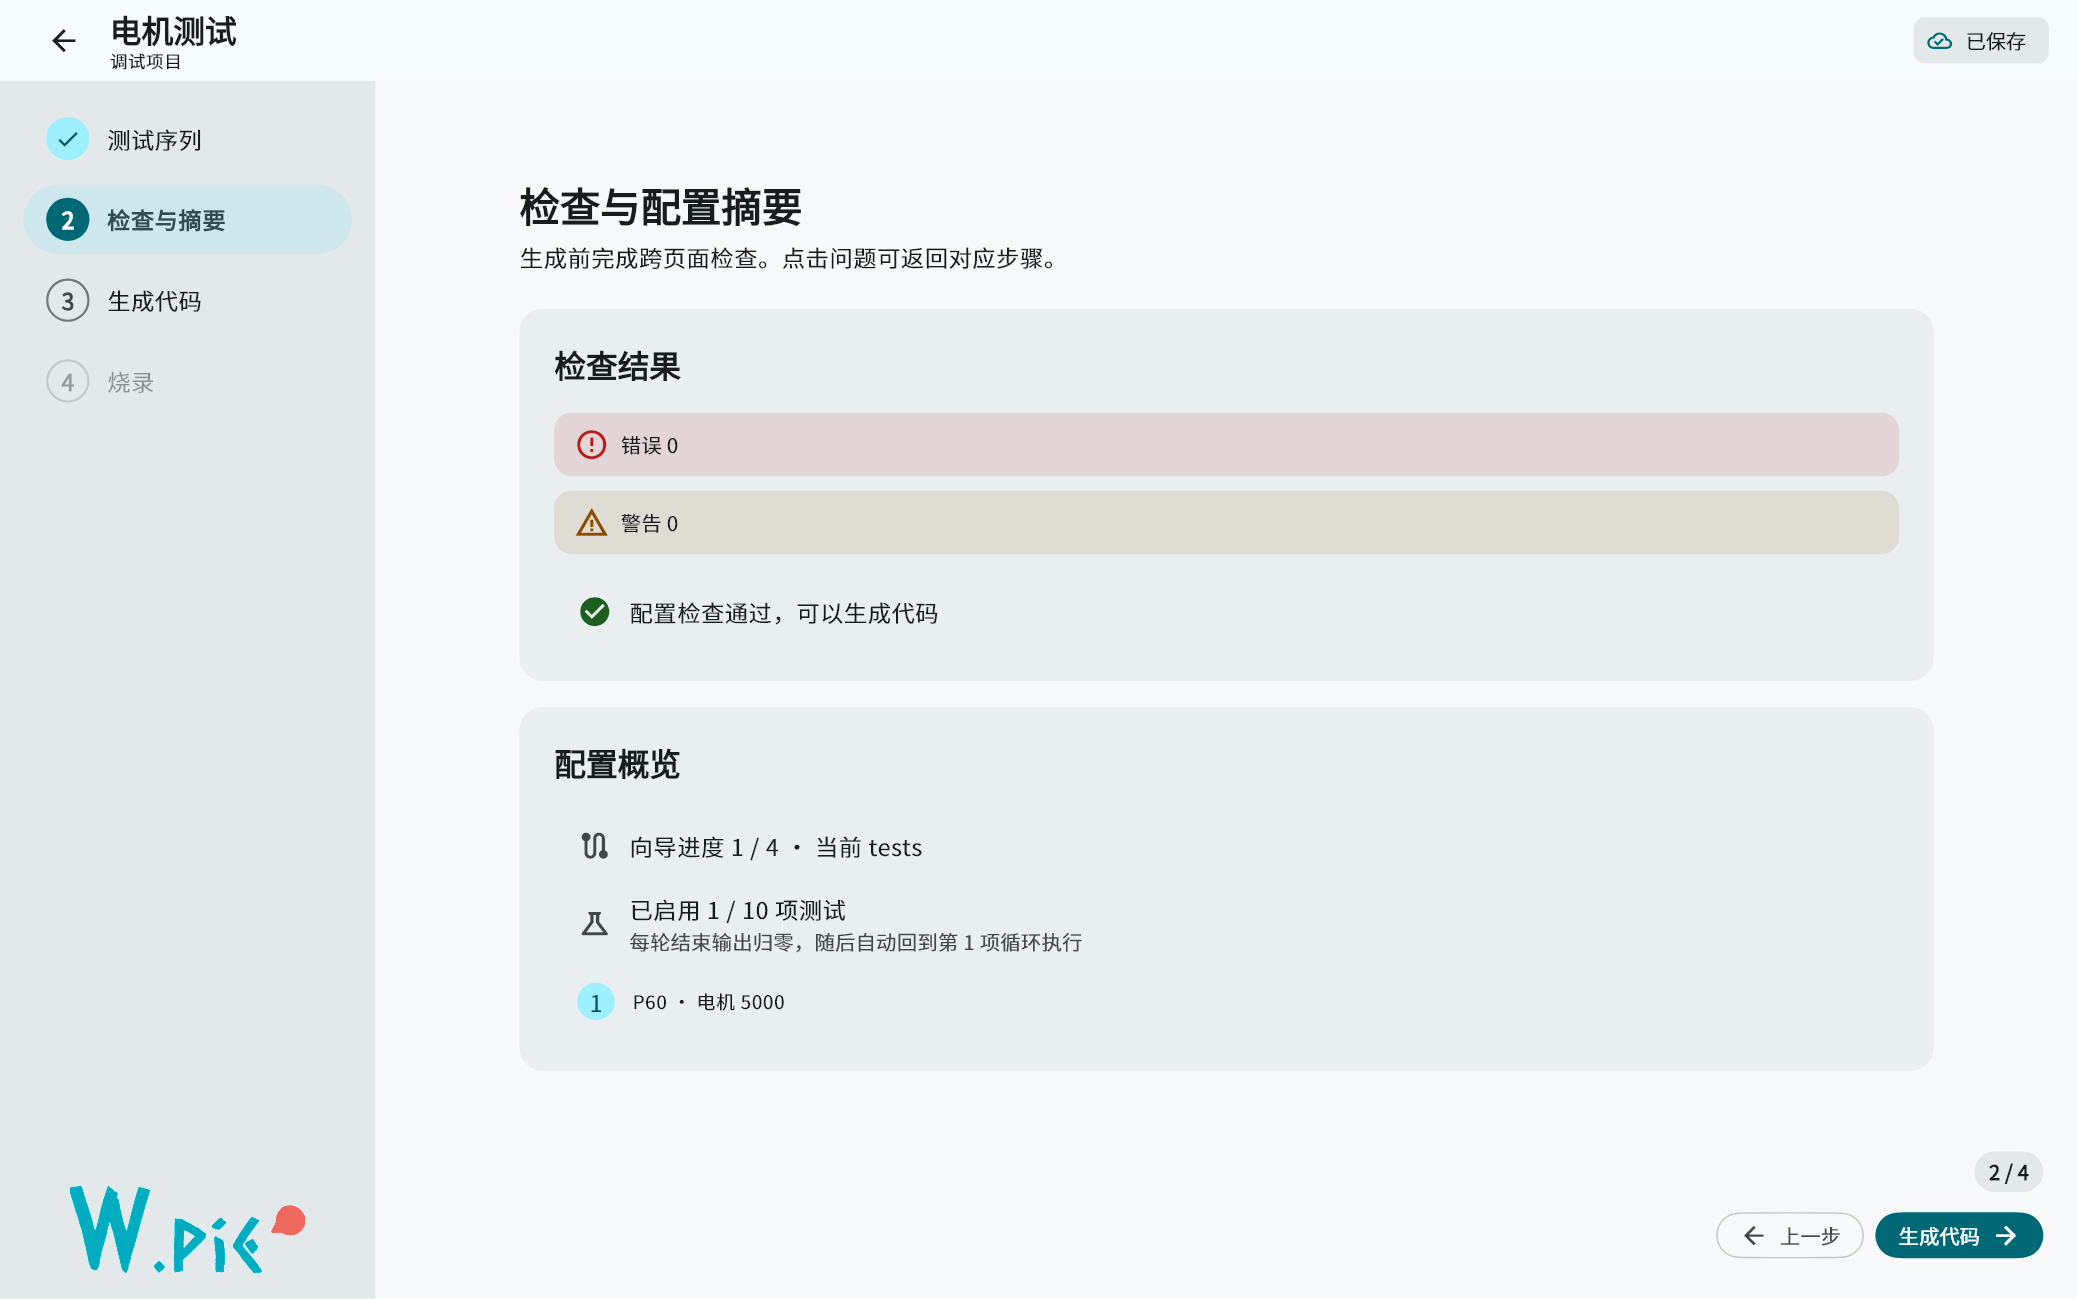
\includegraphics[width=0.95\linewidth]{image/ch02/2-2-review.png}
  \caption{“检查与摘要”页：问题计数与配置概览}
  \label{fig:concise-debug-review}
\end{figure}

“配置概览”汇总已启用的项数与每一项的摘要，供生成前最后核对。若有问题，点击列表中的
条目可直接跳回对应页面；修改后返回检查页，计数随之更新。

\section{编译与烧录}

进入“烧录”页（图~\ref{fig:concise-debug-deploy}）。编译器一栏保持默认的内置编译器即可。
“构建产物”显示编译结果与产物大小；“编译并烧录”完成编译并写入主控板，“仅编译”只验证
配置与编译环境。

\begin{figure}[htbp]
  \centering
  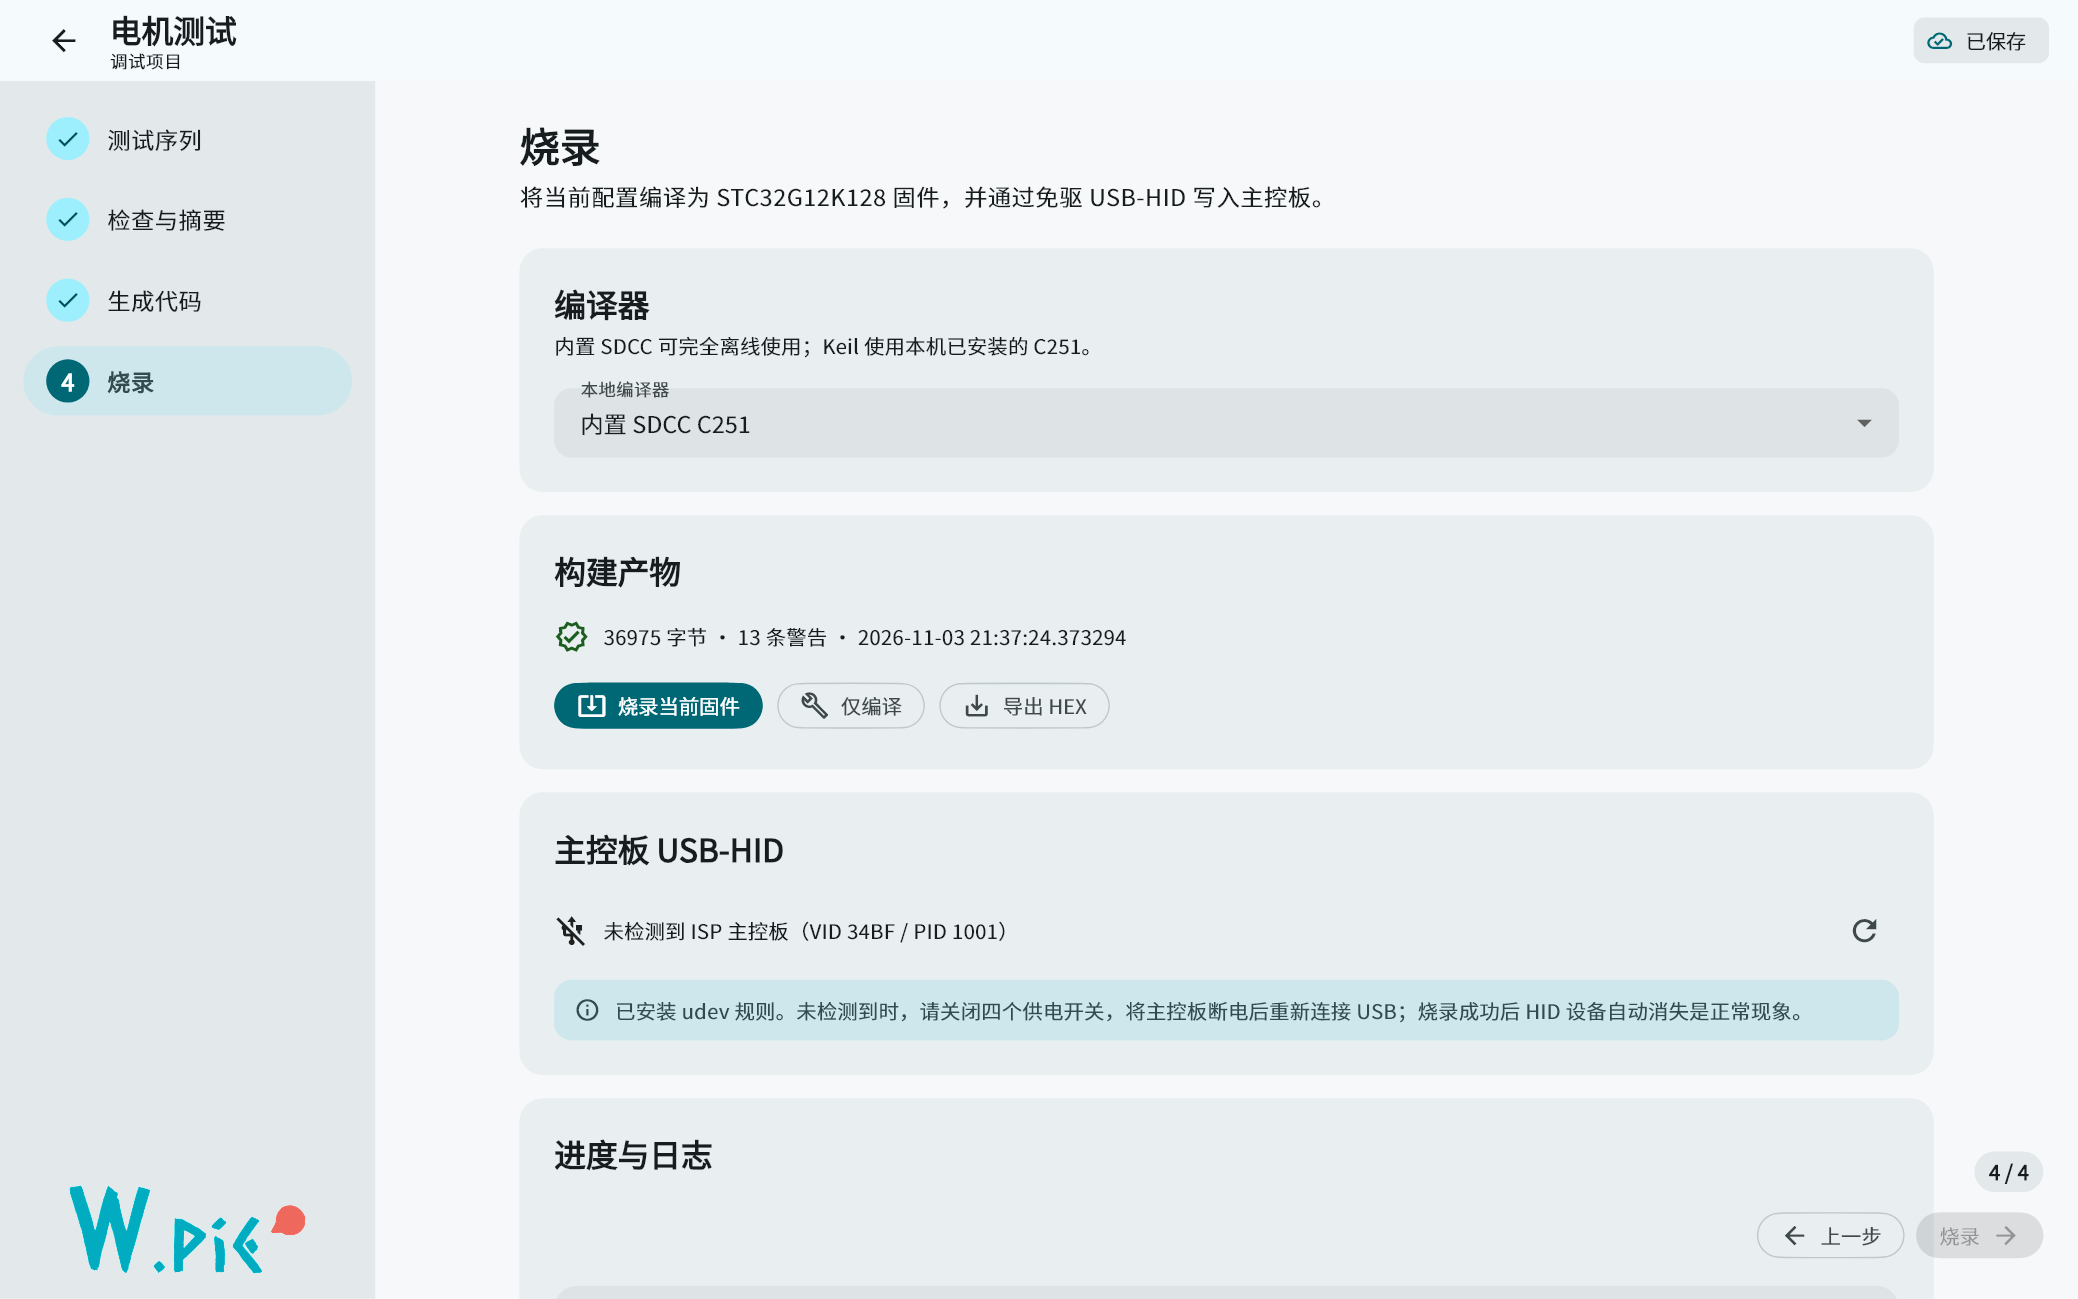
\includegraphics[width=0.95\linewidth]{image/ch02/2-4-deploy.png}
  \caption{“烧录”页：编译器、构建产物、主控板检测与进度日志}
  \label{fig:concise-debug-deploy}
\end{figure}

烧录前完成以下准备：

\begin{enumerate}
  \item 关闭主控板 SERVO、POWER 与机械拓展板 POWER、BOOSTER 四个供电开关；
  \item 将主控板断电，再通过 USB 连接电脑并重新上电，使其进入烧录状态；
  \item 页面检测到主控板后，“编译并烧录”按钮可用。
\end{enumerate}

烧录过程中的进度与日志显示在页面下方。烧录成功后设备会自动复位，检测到的烧录设备消失，
属于正常现象。再次烧录前需要重新断电、上电。

\begin{note}
只能烧录主控板。机械拓展板不运行用户固件，向拓展板烧录会破坏其出厂程序。
\end{note}

\section{上电观察}

烧录完成后接通电源，主控板播放启动提示音，随后按测试序列逐项执行。观察要点：

\begin{itemize}
  \item 每一项是否按设定的方向与时长动作，结束后是否停止；
  \item 提示音的个数是否与当前项序号一致；
  \item 跑完最后一项后是否自动回到第 1 项循环。
\end{itemize}

若某一项方向相反，回到测试序列把该项数值改为相反的符号，重新编译烧录即可，不需要
更改接线。若某一项完全不动作，依次检查供电开关、接线与烧录是否成功。调试项目不使用
遥控器，因此不涉及通道号与死区。
